%!TEX TS-program = xelatex
%!TEX encoding = UTF-8 Unicode
\documentclass[11pt,a4paper]{article}

\usepackage[left=80pt,top=60pt,bottom=110pt,right=60pt]{geometry}
\usepackage{amsmath}
\usepackage{amsfonts}
\usepackage{amssymb}
\usepackage{fixltx2e}
\usepackage{cmap}
\usepackage{enumerate}
\usepackage{ifthen}
\usepackage{listings}
\usepackage{url}
\usepackage[T1]{fontenc}
%\usepackage{fontspec}
%\usepackage{xunicode}
%\usepackage{xltxtra}
%\setmainfont[Mapping=tex-text,Ligatures={Common,Rare,Discretionary}]{Linux Libertine O}
\usepackage{pdflscape}
\usepackage{alltt}
\usepackage{algpseudocode}
\usepackage{subfigure}
\usepackage{graphicx}
\usepackage{verbatim}

\ifthenelse{\isundefined{\hypersetup}}{
    \usepackage[colorlinks=true,linkcolor=blue,urlcolor=blue]{hyperref}
    \urlstyle{same}
}{}

\hypersetup{
    pdftitle={Intelligent Agents - EX3 - Yoan Blanc, Tiziano Signo}
}
\title{\phantomsection%
    A Centralized Agent for the Pickup and Delivery Problem
}
\author{
    \textbf{Group 16}\\
    Yoan Blanc \texttt{<yoan.blanc@epfl.ch>}, 213552\\
    Tiziano Signo \texttt{<tiziano.signo@epfl.ch>}, 226511
}
\date{\today}


\begin{document}
\maketitle

\noindent
\begin{quote}{\it

    In this exercise you will implement the Stochastic Local Search algorithm
    (SLS) to find an efficient solution to the CSP description of the PDP.

    \begin{enumerate}
        \item Implement the Stochastic Local Search algorithm for the PDP.

        \item Run simulations for different configurations of the environment
        (i.e. different tasks and number of vehicles) in order to observe the
        behavior of the centralized planner using the SLS algorithm.

        \item Reflect on the fairness of the optimal plans. Observe that
        optimality requires some vehicles to do more work than others.
        Illustrate this observation with an example in your report.

        \item Test your program for different number of vehicles and various
        sizes of the task set. How does the complexity of your algorithm depend
        on these numbers?

    \end{enumerate}

}\end{quote}

\newpage
\section*{Implementation}

The system is composed of $N_T$ tasks that has to be picked up from a city
and delivered to another city. There is $N_V$ vehicles that are carrying a
schedule to handle a subset of the tasks.

\subsection*{State representation}

Every task $t_i$ is split into two actions: $p$ (pickup) and $d$ (delivery).

\begin{align*}
actions = \{&t_1^p,                               & \text{task $1$ pickup} \\
            &t_1^d,                               & \text{task $1$ delivery} \\
            &t_2^p, \: t_2^d,                     & \text{task 2} \\
            &\dots,                               & \\
            &t_{N_T}^p, t_{N_T}^d\}               & \text{up to the end}
\end{align*}

The set of schedules (the plan) is formed of tuples, one per vehicle, and the
corresponding list of actions to do.

\begin{align*}
plan = \{&\langle v_1, (t_j^p, t_j^d, \: \dots) \rangle,            & \text{vehicle $1$ and task $j$} \\
         &\langle v_2, (t_k^p, t_l^p, \dots, t_k^d, t_l^d) \rangle, & \text{interleaved tasks} \\
         &\dots,                                                        & \\
         &\langle v_{N_V}, \varnothing \rangle\}                    & \text{actions can be empty too}
\end{align*}

There is strong constraints that:

\begin{enumerate}
    \item two actions belonging to a task must be in the same schedule,

    \item pickup and delivery must appear in that order,

    \item every possible action appears once and only once in the plan,

    \item at no time the loaded tasks total weight exceeds the vehicle capacity.
\end{enumerate}


\subsection*{Algorithm}
\subsubsection*{\textsc{initialSolution}}

We've played with two strategies for the \textsc{initialSolution} part:

\begin{enumerate}
    \item \textbf{All tasks to the biggest agent}\\
        This solution seems to converge quickly and give better solution
        overall. The downside is that it has no incentives to split the tasks
        among other vehicles. (See \emph{Fairness} below)

    \item \textbf{Round-robin assignement of tasks}\\
        This solution usually gives worse result than the previous all-to-one
        idea but enlighten why better solutions require less agent. Hence, we
        didn't keep it as the default way of populating the initial schedules.

\end{enumerate}


\subsubsection*{\textsc{chooseNeighbors}}

Instead of doing two things (like in the documentation given): moving one task
from one schedule to another one and reorder one schedule. It's computing all
the possible positions across all schedules for a task. To do so, the task is
removed from the plan and the inserted at the acceptable positions (without
taking care of the vehicle's capacity).

If a schedule has $t$ tasks, there is $(2t - 1)t$ different positions. The
overall cost is $O(|N_V| \cdot (\frac{|N_T|}{|N_V|})^2) \approx O(|N_T|^2)$ which was
expected.


\subsection*{\textsc{localChoice}}

For the last part and certainly not the least, three things were explored:

\begin{enumerate}
    \item \textbf{Greedy local search}
        The more straightforward algorithm which keeps the best solution. It'll
        remain stuck in a local maxima in most cases. Good solutions may be
        found with it but it requires many retries.

    \item \textbf{Stochastic local search}
        The search keeps all the better ones and randomly picks one from them.
        It won't converge as quickly as the greedy one and should be less
        likely stuck into premature local maxima. The results are comparable
        to the \textbf{greedy} one though.


    \item \textbf{Simulated annealing}
        Because this one can escape from a local maxima it tends to find better
        solutions most of the time. That's the one we'll use for the evaluation.

        It seemed that the \textsc{initialSolution} picked had no impact on it
        like it does for the two previous one.

\end{enumerate}


\section*{Behaviour}

Since the only factor is the money spend travelling here, the algorithm tends
to assign all the tasks to one agent. More details in the next section.


\section*{Optimality \& Fairness}

\subsection*{Optimality}

Optimality means travelling a very few to deliver a maximum stuff. A way to
look at it is the display the load over time (or travelling distance). We see
in Figures~\ref{fig:30_1} and \ref{fig:60} that the final plan try to be on
\textbf{high load} as often as possible.

\begin{figure}[ht!]
    \begin{center}
    \subfigure[Initial state]{
        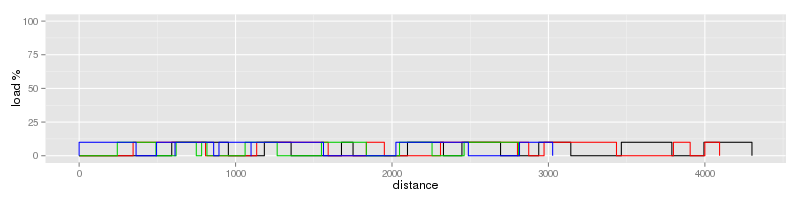
\includegraphics[width=.8\textwidth]{plan_2356_0.png}
        \label{fig:30_0}
    }
    \subfigure[Final state]{
        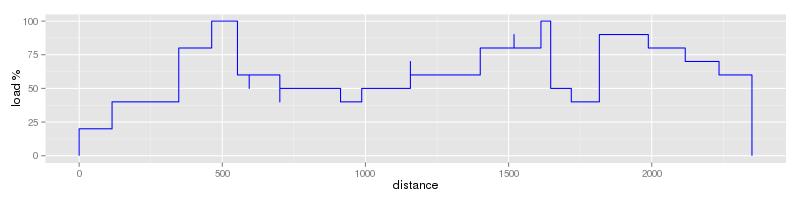
\includegraphics[width=.8\textwidth]{plan_2356_1.png}
        \label{fig:30_1}
    }
    \caption{
        Round-robin distribution of $30$ tasks using \textbf{simulated annealing}
    }{
        Total distance travelled: $2356$ km
    }
    \label{fig:30}
    \end{center}
\end{figure}

\begin{figure}[ht!]
    \begin{center}
    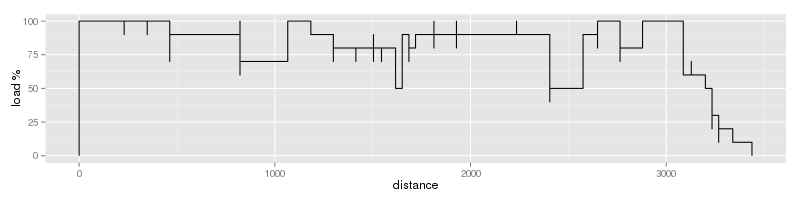
\includegraphics[width=.8\textwidth]{plan_3449_1.png}
    \caption{
        $60$ tasks to the biggest agent using \textbf{simulated annealing}
    }{
        Total distance travelled: $3449$ km
    }
    \label{fig:60}
    \end{center}
\end{figure}


\subsection*{Fairness}

Regarding the fairness, it's not fair as the algorithm tends to reduce the
number of vehicles. Even with the round robin initial setup (see
Figure~\ref{fig:30_0}), the output solution
kept only one vehicle and it's not load most of the time. For the $60$ task
example though (Figure~\ref{fig:60}), the system managed to get directly to full
load and to keep being loaded up to the end.

One explanation to this is that for every vehicle there is:
\begin{itemize}
    \item a \emph{loading up} phase where it's collecting tasks to be delivered
        (maximizing the reward per km) at the beginning

    \item and an \emph{unloading} one at the end.

\end{itemize}

Only the core of the vehicle's schedule where its load is maximized approaches
an optimal solution. Adding more vehicles does not help being on maxmimal load
ideally all the time.


\section*{Algorithm complexity}

As explained before, the complexity is of $O(|N_T|^2)$ for each step and does not
depend on the number of vehicles. The \textbf{stochastic} and the
\textbf{simulated annealing} are converging much more slower and thus creating
more work but there is no changes in the general order of complexity.


\section*{Conclusion}

Once again, having a way to visualize the results was of great help and lead us
to better understand intermediate results and behaviours. The simulated
annealing wasn't part of the homework but it seemed to be a natural fit here
and proved to indeed be.

\end{document}
